%% -*- coding: utf-8 -*-
\documentclass[12pt,a4paper]{scrartcl} 
\usepackage[utf8]{inputenc}
\usepackage[english,russian]{babel}
\usepackage{indentfirst}
\usepackage{misccorr}
\usepackage{graphicx}
\usepackage{amsmath}
\begin{document}
	\begin{titlepage}
		\begin{center}
			\large
			МИНИСТЕРСТВО НАУКИ И ВЫСШЕГО ОБРАЗОВАНИЯ РОССИЙСКОЙ ФЕДЕРАЦИИ
			
			Федеральное государственное бюджетное образовательное учреждение высшего образования
			
			\textbf{АДЫГЕЙСКИЙ ГОСУДАРСТВЕННЫЙ УНИВЕРСИТЕТ}
			\vspace{0.25cm}
			
			Инженерно-физический факультет
			
			Кафедра автоматизированных систем обработки информации и управления
			\vfill

			\vfill
			
			\textsc{Отчет по практике}\\[5mm]
			
			{\LARGE \textit{Найти определитель матрицы}}
			\bigskip
			
			1 курс, группа 1УТС
		\end{center}
		\vfill
		
		\newlength{\ML}
		\settowidth{\ML}{«\underline{\hspace{0.7cm}}» \underline{\hspace{2cm}}}
		\hfill\begin{minipage}{0.5\textwidth}
			Выполнил:\\
			\underline{\hspace{\ML}} О.\,Д.~Козырев\\
			«\underline{\hspace{0.7cm}}» \underline{\hspace{2cm}} 2021 г.
		\end{minipage}%
		\bigskip
		
		\hfill\begin{minipage}{0.5\textwidth}
			Руководитель:\\
			\underline{\hspace{\ML}} С.\,В.~Теплоухов\\
			«\underline{\hspace{0.7cm}}» \underline{\hspace{2cm}} 2021 г.
		\end{minipage}%
		\vfill
		
		\begin{center}
			Майкоп, 2021 г.
		\end{center}
	\end{titlepage}
		
	\section{Введение}
	\label{sec:intro}
	\begin{enumerate}
	\item Текстовая формулировка задачи:
	
	Найти определитель матрицы.
	\item Код на языке C++ приведен в пункте~\ref{sec:exp:code} на стр.~\pageref{sec:exp:code}.
	\item Результат работы представлен в пункте~\ref{sec:result:screen} на стр.~\pageref{figure:screen}.
	\end{enumerate}
	
	\section{Ход работы}
	\label{sec:exp}
	
	\subsection{Код программы}
	\label{sec:exp:code}
	\begin{verbatim}
	
#include <iostream>
#include <locale>
using namespace std;
int main() {
    setlocale(LC_ALL, "rus");
    int n;
    double tmp, d;
    cout << "Введите размерность матрицы:\n";
    cout << "n = ";
    cin >> n;
    double** a = new double* [n];
    for (int i = 0; i < n; i++) {
        a[i] = new double[n]; }
    cout << "Введите матрицу:\n";
    for (int i = 0; i < n; i++) {
        for (int j = 0; j < n; j++) {
            cin >> a[i][j]; } }
    for (int k = 0; k < n - 1; k++) {
        for (int i = k + 1; i < n; i++) {
            tmp = -a[i][k] / a[k][k];
            for (int j = 0; j < n; j++) {
                a[i][j] += a[k][j] * tmp; } } }
    cout << "\nМатрица:\n\n";
    cout.precision(2);
    for (int i = 0; i < n; i++) {
        for (int j = 0; j < n; j++) {
            cout.width(8);
            cout << fixed << a[i][j] << " "; }
        cout << "\n"; }
    d = 1;
    for (int i = 0; i < n; i++) { d *= a[i][i]; }
    cout << fixed << "\nОпределитель: " << d << "\n";
    for (int i = 0; i < n; i++) { delete[] a[i]; }
    delete[] a;
    system("pause");}
	
	\end{verbatim}
	
	\section{Результат работы программы}
	\label{sec:result}
	
	\subsection{Скриншоты выполнения кода}
	\label{sec:result:screen}
	\begin{figure}[h]
	\centering
	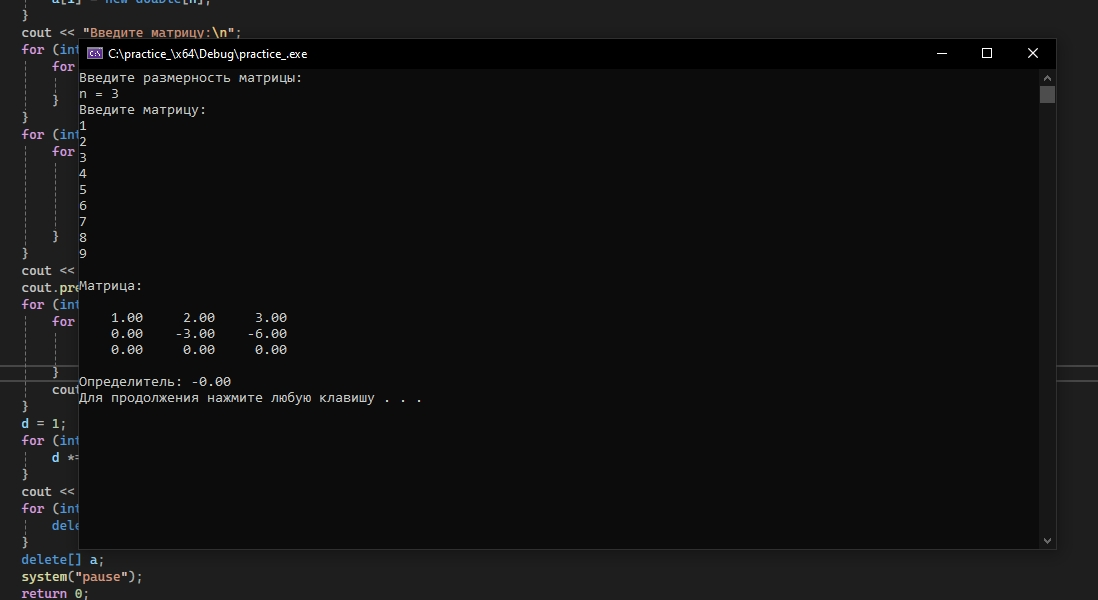
\includegraphics[width=1\textwidth]{skrin.jpg}
	\caption{Окно вывода программы}\label{figure:screen}
	\end{figure}

	\begin{thebibliography}{9}
	\bibitem{Knuth-2003}Кнут Д.Э. Всё про \TeX. \newblock --- Москва: Изд. Вильямс, 2003 г. 550~с.
	\bibitem{Lvovsky-2003}Львовский С.М. Набор и верстка в системе \LaTeX{}. \newblock --- 3-е издание, исправленное и дополненное, 2003 г.
	\bibitem{Voroncov-2005}Воронцов К.В. \LaTeX{} в примерах. 2005 г.
	\bibitem{Shildt-2013}Шилдт Г. С++ для начинающих. Шаг за шагом //ЭКОМ Паблишерз. – 2013. – №. 2. – С. 640.

	\end{thebibliography}
	
\end{document}
